%% The following is a directive for TeXShop to indicate the main file
%%!TEX root = ../diss.tex

\chapter{Oxygen enhanced MRI}
\label{ch:oemri}

\section{Preface}

Stuff about contributions 

% ======================================================================
% Abstract
% ======================================================================
\section{Abstract}
\textbf{hypoxia; oxygenation; oxygen enhanced MRI; tumours; } % 3-6 keywords

\textbf{Purpose}: This study improves the sensitivity and speed of existing oxygen enhanced MRI (OE-MRI) techniques.
We demonstrate broad applicability of dynamic oxygen enhanced MRI (dOE-MRI) in multiple tumour models and evaluated its reliability and speed.

\noindent\textbf{Methods}: Mice were implanted with SCCVII, HCT-116, BT-474, or SKOV3 tumours in the dorsal subcutaneous region and imaged on a 7T scanner.

During the dOE-MRI sequence, a respiratory challenge was administered and mice alternated between breathing medical air and 100\% oxygen every 2 minutes for a total of 3 cycles.
Data were analyzed with independent component analysis (ICA) and oxygenation maps were generated and compared to corresponding histology sections.
Tumours were excised and stained for hypoxia (pimonidazole), blood vessels (CD31), perfusion (Hoechst or carbocyanine) following imaging.

\noindent\textbf{Results}: Presence of physiological noise, signal drift, and temperature variability have a much larger impact on T$_1$-w signal intensity than oxygen inhalation.
However use of ICA permitted the extraction of the oxygen enhancing component in all imaged tumours across four different tumour lines with varying oxygenation statuses.
Additionally, dOE-MRI does not require a priori knowledge of the response function and the technique is sensitive enough to assess temporal variability of response in individual oxygen cycles.
Spatial parameter maps obtained from dOE-MRI correspond to matched histology sections, particularly well-oxygenated (dOE-MRI, O$_2$-positive) and pimonidazole-negative (histology) regions.
Using ICA and adding a cycling gas challenge to OE-MRI extends the sensitivity of the technique beyond only highly perfused tumours and the oxygenation status can be assessed in as little as 6 minutes.

\noindent\textbf{Conclusion}: dOE-MRI presents significant improvements to the sensitivity and applicability of dOE-MRI, making it more clinically relevant and feasible.

% ======================================================================
\section{Introduction}
% ======================================================================

Hypoxia is a well-established component of the tumour microenvironment, arising most often as tumour cell growth outpaces the growth of new vasculature.
Tumour hypoxia is an indicator of poor prognosis and is responsible for tumour resistance to radiotherapy and some chemotherapies, but is also a potentially useful target for novel anti-cancer drugs~\cite{Wilson:2011jp}.
Assessing tumour hypoxia in the clinical setting is challenging largely due to the invasive nature of some biopsy-dependent techniques and the limited capacity and high expense of the more favoured, non-invasive PET imaging~\cite{Horsman:2012kw}.
The utility of screening patients for hypoxia in trials of hypoxia-targeting drug trials was demonstrated retrospectively in trials of the bioreductive hypoxic cytotoxin tirapazamine, where those patients with greater PET-imaged hypoxia experienced greater benefit~\cite{Rischin:2006fz}.
However, subsequent trials of drugs targeting hypoxia, including those for evofosfamide that failed to show clinical benefit, did not use hypoxia imaging for patient stratification.
An alternative, practical, widely applicable, non-invasive imaging-based method is urgently required for monitoring tumour hypoxia in many contexts and is crucial to the development and clinical evaluation of future hypoxia-targeting drugs.

As early as 1981, the T$_1$ shortening property of inhaled oxygen has been known~\cite{Young:1981vf,Thulborn:1982tb} and there is no doubt in the MR imaging community that tissue oxygenation has a subtle but measurable influence on T$_1$ as shown in many independent studies by O'Connor~\cite{OConnor:2016ee,OConnor:2009ku,OConnor:2009bp}, Mason~\cite{Zhao:2015ez,White:2016fz,Hallac:2014cb}, Gallez~\cite{Jordan:2012do}, and others~\cite{Tadamura:1997vc,McGrath:2008kx,Kershaw:2010ha,Linnik:2013hf}.

Oxygen-enhanced MRI (OE-MRI) detects the shortening of the T$_1$ relaxation time that occurs in tissues when oxygen concentrations dissolved in fluids increase as a result of breathing excess oxygen.
This T$_1$-shortening effect is similar, though of much smaller magnitude, to that of paramagnetic, Gd-containing contrast agents.
While OE-MRI measurements do not depend directly on exogenous contrast agents, nor do they require specialized MR acquisition techniques, OE-MRI has not found routine clinical use largely because of challenges quantifying T$_1$ due to its low sensitivity, particularly in any tumour model that is not highly vascularized~\cite{OConnor:2016ee, Zhao:2015ez}.
This has been overcome by performing DCE-MRI alongside OE-MRI to separate perfused voxels from non-perfused voxels, enabling improved isolation of the oxygen-induced T$_1$ signal.
Recent OE-MRI efforts at The Christie NHS Foundation Trust in Manchester and Institute of Cancer Research in London are encouraging {OConnor:2016ee} but wide application may still be limited as the technique continues to have signal-to-noise constraints [personal communication] and long imaging times upwards of 40 minutes.

A technique that is fast, flexible, affordable, repeatable, non-invasive, and requires no injectable contrast agent to measure tumour oxygenation has the potential to significantly impact the clinical fields of radiation biology and hypoxia drug targeting.
In this study, we present a new dynamic OE-MRI (dOE-MRI) technique that is fast and allows extraction of very small dynamic signal changes in T$_1$-weighted (T$_1$-w) images by deliberate induction of multiple step changes in the inspired oxygen through a repeated, cycling gas challenge.
We further use independent component analysis (ICA), a machine-learning approach, to extract independent signal components within the tissues that match the gas cycling challenge.
With the application of a cycling oxygen challenge and processing the data using ICA, our dOE-MRI approach represents a significant improvement in the sensitivity and application of MRI for measuring tumour oxygenation, making it more practical for wide clinical application.


% ======================================================================
\section{Methods}
% ======================================================================
\subsection{Mice and tumours}

Female NRG mice were bred and housed in institutional animal facilities; experiments in this study were approved by the Animal Care Committee of the University of British Columbia.
Animals were implanted with murine squamous cell carcinoma SCCVII tumours (cells provided by Dr. J Evans) or with human colorectal carcinoma HCT-116, human ovarian carcinoma SKOV3 or human breast carcinoma BT474 tumours (obtained from the American Type Culture Collection) and were imaged when the largest tumour diameters reached approximately 8-10 mm.

Mice were anesthetized with isoflurane for the duration of imaging sessions until euthanasia, and were positioned supine on the custom surface coil apparatus.
Continuous monitoring of respiration rate, varying between 80-100 breaths per minute, and body temperature, maintained at 37 $\pm$ 0.5$^\circ$C using a continuous airflow heater, were performed throughout the imaging session.
All animals were injected with 60 mg/kg pimonidazole hydrochloride (HypoxyProbe)  30 min prior to imaging to label hypoxic cells.
One SCCVII tumour-bearing mouse was catheterized and injected with 30mM solution of Gd-DTPA for DCE-MRI at a rate of 1mL/min using a power injector at a dose of 5$\mu$L/g.

Following the imaging sessions, animals were administered a 50 $\mu$L intravenous dose of 2.5 mg/mL Hoechst 33342 (bisbenzimide; ThermoFisher, Waltham, MA, USA) to label the perivascular cell nuclei of perfused vessels, and were euthanized within 15 min of imaging completion. 
Tumours were embedded and frozen in optimum cutting temperature medium (OCT; Tissue-TEK).

\subsection{Immunohistochemistry}

Cryosections, staining, imaging and image processing were performed similarly to as previously reported ~\cite{Baker:2015co}.
Briefly, serial-step 10 $\mu m$ cryosections were cut at 0.5-mm intervals along the same MR imaging plane.
Sections were imaged for Hoechst 33342 fluorescence (380nm), fixed in acetone-methanol for 10 min then whole sections were stained with Hoechst 33342 to label all nuclei and immunohistochemically stained for CD31-labeled blood vessels and pimonidazole-labeled hypoxic cells that were visualized using Alexa 647nm and Alexa 488nm secondary antibodies respectively.
Whole-tumour sections were imaged for each label in greyscale at a resolution of 1.5 $\mu m$/pixel, with images later converted to false colours and overlaid for qualitative analysis.

\subsection{Data Acquisition}
All MRI experiments were performed at the UBC MRI Research Centre on a 7T Bruker BioSpec 70/30 scanner at room temperature with a volume transmit coil and custom surface receive coil.
Each imaging session began with pilot scans for slice prescription and axial RARE images for anatomical reference and localization of the tumour.
Eight slices (1mm thickness) with an in-plane field of view of 3.84 cm x 1.92 cm were acquired with a matrix of 128 x 64.
Dynamic oxygen enhanced MRI (dOE MRI) scans were acquired with a 2D FLASH-based sequence with TE/TR = 2.67ms/66.7 ms, $\alpha$ = 40$^\circ$, temporal resolution of 4.3s with 198 repetitions for a total scan time of about 14 minutes.
The above sequence was shortened to 80 repetitions and also used for the DCE-MRI scan in one animal.
The spatial resolution and geometry for all scans in the imaging session were matched and an experienced operator outlined the tumour on each slice of the anatomy MR images to construct the region of interest (ROI) for each animal.

\noindent\textbf{Gas challenge during MRI:} Tumour-bearing mice began the dOE-MRI gas challenge breathing medical air and were switched between 100\% oxygen and medical air in two minute intervals.
This paradigm continued for three cycles over a total of fourteen minutes.
Gases were switched manually and each switch took about 5 seconds to complete.


\subsection{Data Analysis}
\textbf{Creating dOE-MRI maps:} A suite of in-house software was developed using the python machine learning library scikit-learn, specifically \texttt{sklearn.decomposition.FastICA} based on the technique described by Hyvarinen~\cite{Hyvarinen:2000vk}.
Independent Component Analysis models the observed data as a vector \textbf{x} whose $n$ elements are the mixtures $x_1(t),\ldots,x _n(t)$, another vector \textbf{s} whose $m$ elements are the source signals (independent components) $s_1(t),\ldots,s _m(t)$, as well as a mixing matrix \textbf{A} with elements $a_{ji}$: \textbf{x}=\textbf{A}\textbf{s}.
The independent components $s_i(t)$ cannot be directly observed nor is the mixing matrix \textbf{A} known.

In this application, dynamically acquired T$_1$-w MR images obtained during the cycling gas challenge are represented by \textbf{x}, the mixing matrix \textbf{A} is interpreted as the voxel weighting factors that when linearly combined with the independent source signals $s_1(t),\ldots, s_m(t)$, reproduces the original MR data.
The number of independent components ($m$) for each dataset is chosen by the operator and  ranged from 4$\ldots$9 for each dataset.
The number was chosen based on best separation of the signal intensity change due to the gas challenge from other changes.
Accordingly, only one of the independent components $s_i(t)$ corresponds to the gas challenge and is identified as the oxygen-enhanced component.

Other independent components include factors that affect T$_1$, including temperature variations, but also structured and physiological noise as well as breathing artefacts.
The associated weighting factors $a_{ik}=a_{i1},\ldots,a_{in}$ are a spatial ICA parameter map, with higher (positive) values corresponding to voxels whose time course exhibits a higher (positive) contribution from the corresponding $k$-th OE component.
The extraction of the independent components is not ordered and while the component selection can be automated, in this study an observer was assigned to select the appropriate component (Figure~\ref{technique}).
A schematic of the typical dOE-MRI workflow is shown in Figure~\ref{workflow}.

\noindent\textbf{Creating the perfusion map:} Signal intensity time course from the DCE-MRI map was first normalized to the mean signal intensity pre-injection.
Area under the first 60 seconds of the normalized signal intensity enhancement curve after the injection was calculated (IAUC$_{60}$) using the composite Simpson's Rule (\texttt{scipy.integrate.simps}).
A binary ground-truth perfusion map was constructed by classifying all voxels with IAUC$_{60} > 0$ voxels as perfused and everything else as unperfused.

\begin{figure}[htbp]
   \centering
   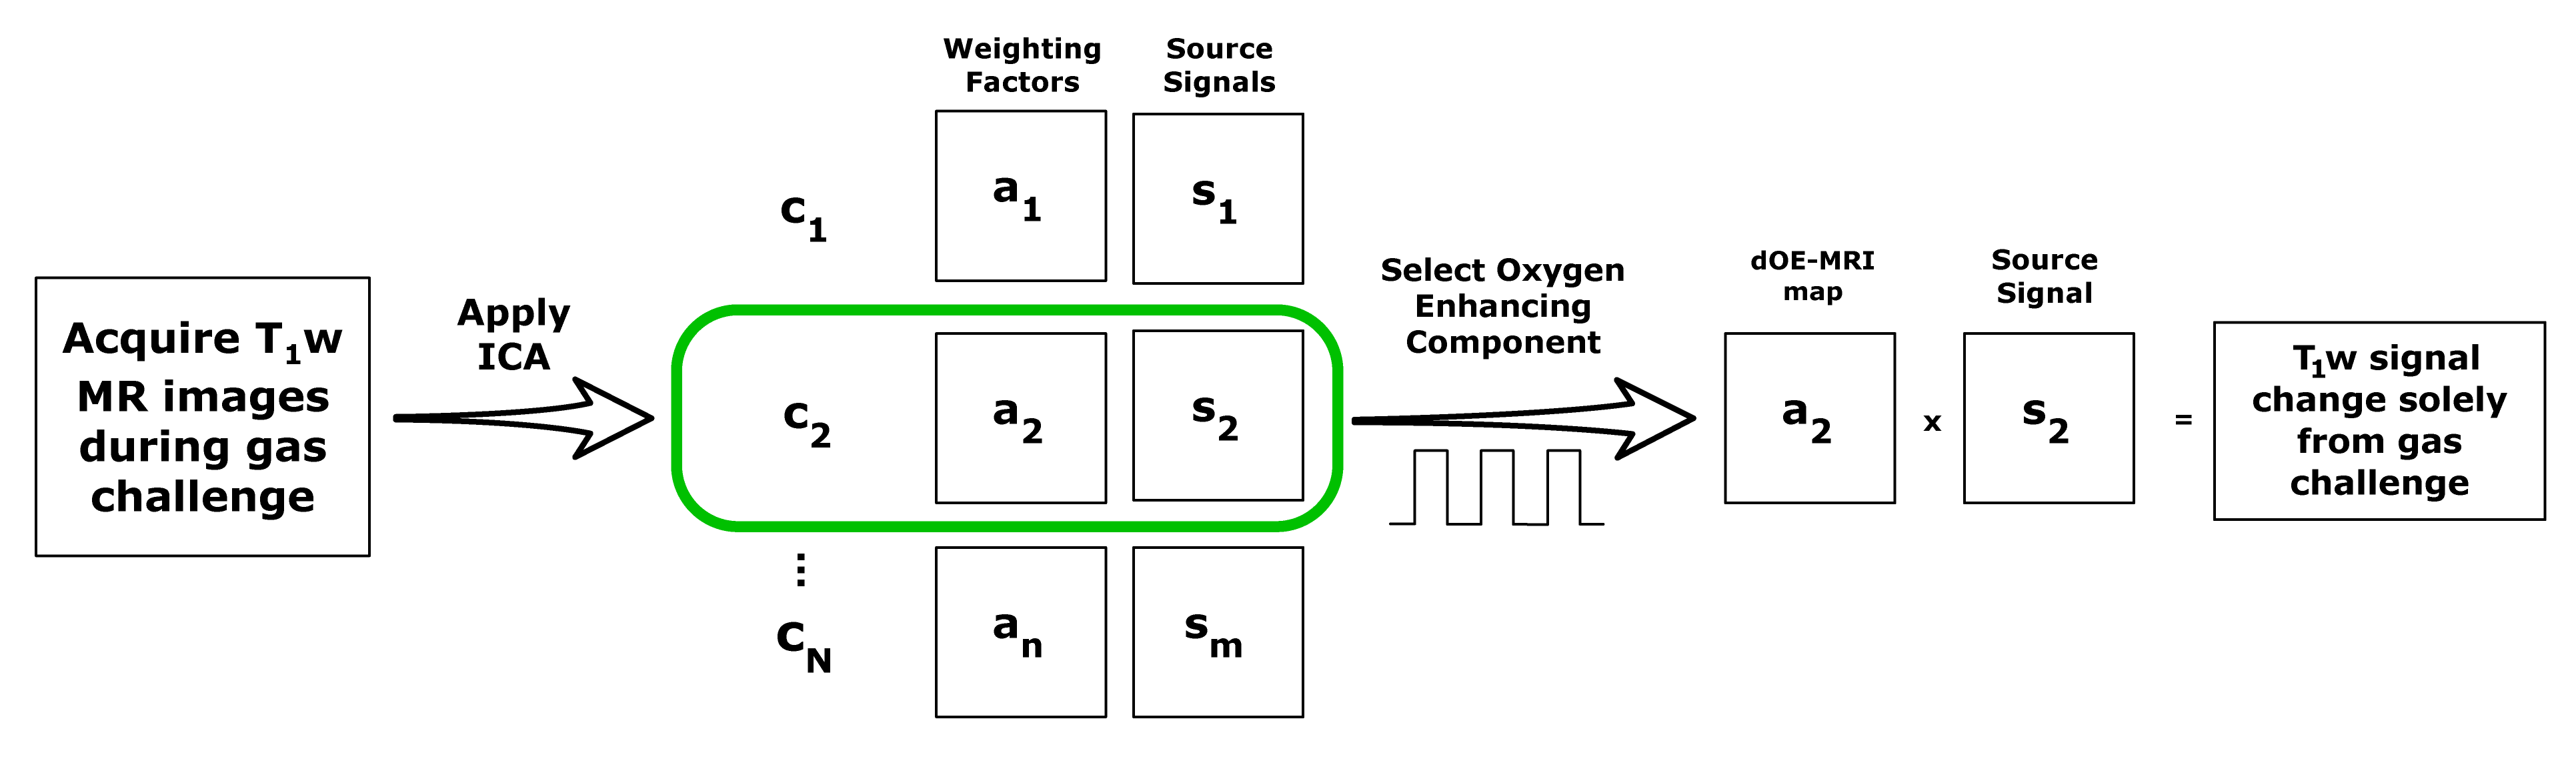
\includegraphics[width=\textwidth]{oemri/oemri-images/oemri_workflow.png} % requires the graphicx package
   \caption{Schematic representation of the dOE-MRI acquisition and analysis technique \textit{in vivo} using ICA.
First T$_1$-weighted images are acquired dynamically with the mice alternatively breathing air or 100\% O$_2$ in 2 minute cycles.
ICA is then applied to the raw data and the data is extracted into a linear combination of $N$ components.
An individual component $c_i$ is captured by a spatial map of weighting factors $a_i$ as well as the corresponding source signal $s_i$.
For the dOE-MRI method, one of the components is selected as the one corresponding to the gas cycle ($c_2$) marked by a green box in this schematic.
Then, $a_2$ is the dOE-MRI map and $s_2$ is the extracted T$_1$-w component by ICA.}
   \label{workflow}
\end{figure}

\noindent\textbf{dOE-MRI without ICA:} To assess whether or not ICA was required to create oxygenation maps, the MR signal intensity data was correlated with three gas paradigms: 1) square wave which corresponds to the concentration of delivered oxygen; 2) a sine wave which models short delays before and after the tumour microenvironment responds to the excess O$_2$ and its removal; and 3) the extracted oxygen-enhancing ICA component.
Correlations were calculated voxel by voxel using:

\begin{equation}
r = \frac{\Sigma^n_{i=1} (x_i - \bar{x}) (y_i - \bar{y})}{\sqrt{\Sigma^n_{i=1} (x_i - \bar{x})^2 \Sigma^n_{i=1} (y_i - \bar{y})^2}}
\end{equation}
where $x$ and $y$ are the model paradigm or the T$_1$-w signal intensity time course.
The resulting correlation maps are estimates of the strength of the input paradigms with the acquired signal intensity.


% ======================================================================
\section{Results}
% ======================================================================

\subsection{ICA isolates small changes in T$_1$-w signal intensity}

An example signal intensity vs.\ time curve is shown for a whole slice ROI compared with a single voxel (Figure~\ref{technique}).
A mean signal intensity increase is seen for both the whole slice and the individual voxel during each of the oxygen periods of the cycle, however the magnitude of change is low for the average and the signal to noise is very poor for the individual voxel.
These data illustrate the relatively poor sensitivity of averaged OE-MRI signal measurements.
ICA was used to extract four independent components from the same whole slice time course of T$_1$-w signal intensity data during the cycling oxygen challenge.
One of the four components clearly corresponds to the periodic switching of oxygen and air.
The unambiguous match of the identified component with the periods of the gas cycles increases the confidence that the small T$_1$-w signal changes result from increased oxygen dissolved in the plasma and interstitial tissue fluids.
    

\begin{figure}[htbp]
   \centering
   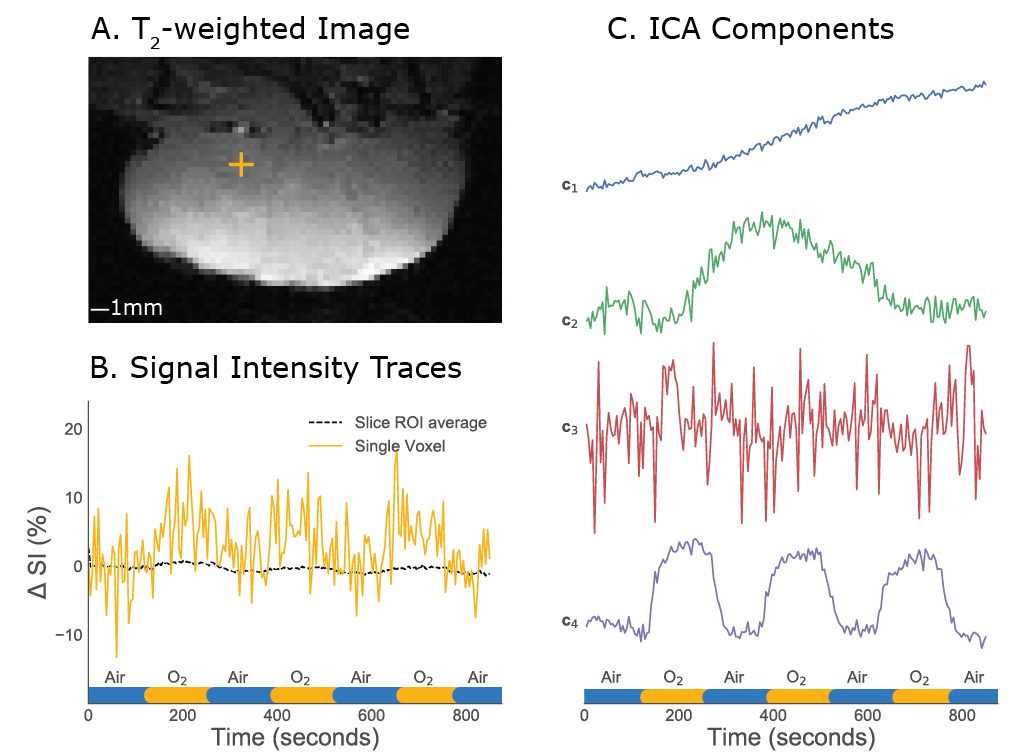
\includegraphics[width=\textwidth]{oemri/oemri-images/oemri_technique.png} % requires the graphicx package
   \caption{(A) T$_2$-weighted MRI of a tumour xenograft at 7T and (B) the corresponding T$_1$-w signal-time traces of a single voxel (solid yellow) and whole-tumour slice ROI (dotted black) during gas cycling at two-minute intervals of air (x axis; blue) and O$_2$ (x axis;yellow).
(C) Plot of 4 extracted ICA components from the entire tumour ROI, component four (\textbf{c$_4$}, purple) corresponds to the periods of oxygen cycling shown on the x axis, and is identified as the component corresponding to the gas challenge.}
   \label{technique}
\end{figure}

\subsection{ICA enabled dOE-MRI detects variable oxygenation in a range of tumour models}

Four tumour models were imaged using dOE-MRI with ICA extraction of the oxygenation component; representative spatial dOE-MRI parameter maps from each tumour type are shown in Figure~\ref{versatile}.
Voxels are coloured to indicate the amount by which a given pixel intensity time course is modulated by the oxygen-related component.

In these dOE-MRI maps, O$_2$-positive voxels (purple) represent an increase in T$_1$-w signal intensity and therefore are thought to correspond to areas with excess dissolved oxygen, while voxels with decreasing T$_1$-w signal intensity under oxygen breathing are termed O$_2$-negative (green).

Tumours include human and murine cell lines with a variety of tumour microenvironments that include fast growing, highly vascularized murine squamous cell (SCCVII) and human ovarian (SKOV3) carcinomas, and slower growing and well vascularized human breast cancer (BT474), as well as a relatively fast growing and more poorly vascularized human colon colorectal carcinoma (HCT-116).
The variable patterns of OE-MRI mapped oxygen distribution reflect the heterogeneous microenvironments of the tumours.


\begin{figure}[htbp]
   \centering
   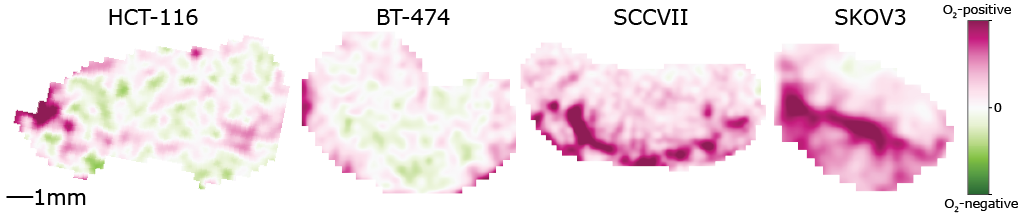
\includegraphics[width=\textwidth]{oemri/oemri-images/oemri_versatile.png} % requires the graphicx package
   \caption{dOE-MRI maps from independent component analysis of four tumour cell lines HCT-116, BT-474, SCCVII, and SKOV3.
Purple marks voxels whose time course exhibits a higher (positive) contribution from the extracted oxygen responsive component.}
   \label{versatile}
\end{figure}

\subsection{dOE-MRI with ICA does not require a priori knowledge of response function}

Oxygenation status maps were also obtained by correlating mathematical representations of the gas challenge with the raw time-signal voxel-by-voxel (Figure~\ref{correlation}A).
A dOE-MRI map generated without prior knowledge of a response function was compared with maps showing voxel-wise correlation of the dynamic image data with response functions square and sine, and temporal component as extracted using ICA.
The regions most correlated with the input paradigm remained purple in all three cases and showed approximately similar demarcated regions of O$_2$-positive and O$_2$-negative, however, the square and sine response functions led to consistent underestimation of oxygenation relative to the dOE-MRI map.
The signal intensity correlation was strongest for the previously extracted ICA component and led to the closest match with the dOE-MRI map.

\begin{figure}[htbp]
   \centering
   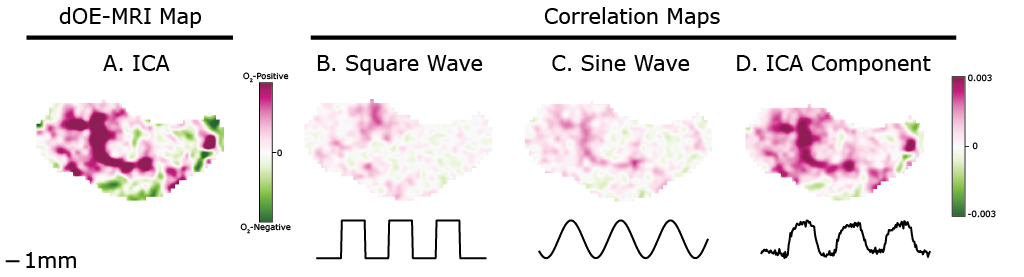
\includegraphics[width=\textwidth]{oemri/oemri-images/oemri_correlation.png} % requires the graphicx package
   \caption{dOE-MRI map (A) of an SCCVII tumour compared to pearson's r-maps obtained by correlating the raw time-signal voxel by voxel with a square wave (B), a sine wave (C), as well as the extracted ICA component (D).
Purple voxels (positively correlated with the model paradigm) indicate an increase in signal intensity following oxygen inhalation.}
   \label{correlation}
\end{figure}

\subsection{Variability of response in individual oxygen cycles}

While a full dOE-MRI sequence involved three cycles of oxygen, to assess the potential for shortening the sequence we also separately applied ICA to each of the three oxygen cycles.
Resulting dOE-MRI maps were compared to the map obtained by applying ICA to all three oxygen cycles together.
Separated dOEMRI maps, as well as voxel-wise correlation plots of a representative SCCVII tumour are shown in Figure~\ref{repeatability} with Pearson's r$_{all-1}$=0.74,r$_{all-2}$=0.86,r$_{all-3}$=0.84.
Pearson's r ranged from 0.79 to 0.87 for a similar analysis in a representative HCT-116 tumour.
This shows that an individual oxygen cycle (about 6 min) is sufficient to map tissue oxygenation.

Another dOE-MRI map was generated to evaluate general stability of the ICA component extraction process by undersampling the full time course threefold (Figure~\ref{repeatability}E) and correlating that with the full dOE-MRI map resulted in Pearson's r = 0.84.
The comparison of this correlation to that of the individual cycles above shows the stability of the technique and illustrates how a benchmark for oxygen-status variability should be constructed.
Neither the SCCVII (Figure~\ref{repeatability}) nor the HCT-116 tumours (data not shown) had significant, measurable changes in oxygenation over the imaging time of 14 minutes.


\begin{figure}[htbp]
   \centering
   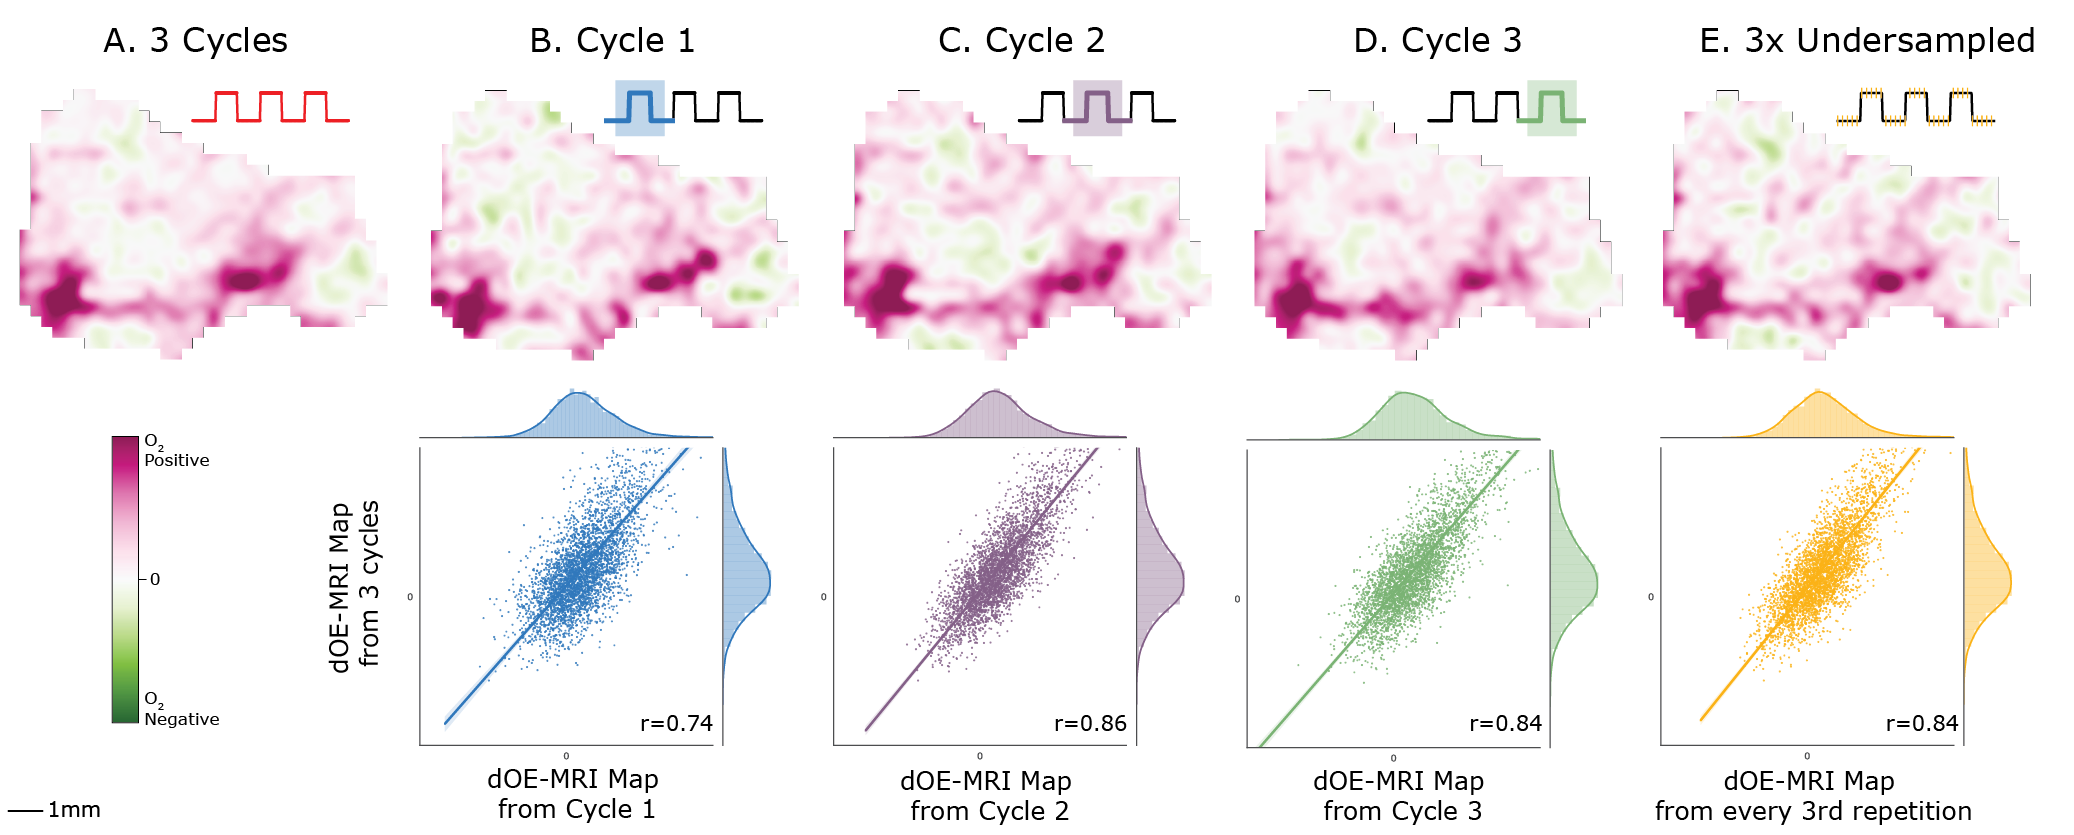
\includegraphics[width=\textwidth]{oemri/oemri-images/oemri_repeatability.png} % requires the graphicx package
   \caption{Demonstrating the versatility of the technique, dOE-MRI maps were generated with each of the gas cycle challenges separately.
The dOE-MRI maps from all three cycles (A) are compared to each of the three gas cycles (B,C,D respectively) with voxel-wise plots of each map correlated to the full dataset shown along with a linear regression with pearson's r.
The final map (E) was generated by undersampling and selecting every third datapoint from the full dataset.}
   \label{repeatability}
\end{figure}

\subsection{dOE-MRI as a surrogate for contrast agent-dependent perfusion imaging}

Where dOE-MRI and DCE-MRI scans were acquired in the same SCCVII tumour-bearing mouse, a map of oxygenation status was compared to an IAUC$_{60}$ perfusion map, both of which are shown in Figure~\ref{perfusion}.
A striking correspondence is observed between the two parameter maps, where highly oxygenated, O$_2$-positive regions generally correspond to the most well perfused, high IAUC$_{60}$ areas of tumour.
To quantitatively evaluate the dOE-MRI map as a surrogate for exogenous contrast-agent perfusion, an ROC analysis was conducted and is shown in Figure~\ref{perfusion}C with an area under the curve of 0.73, suggesting a potentially useful correlation between the two MRI modes of imaging.

\begin{figure}[htbp]
   \centering
   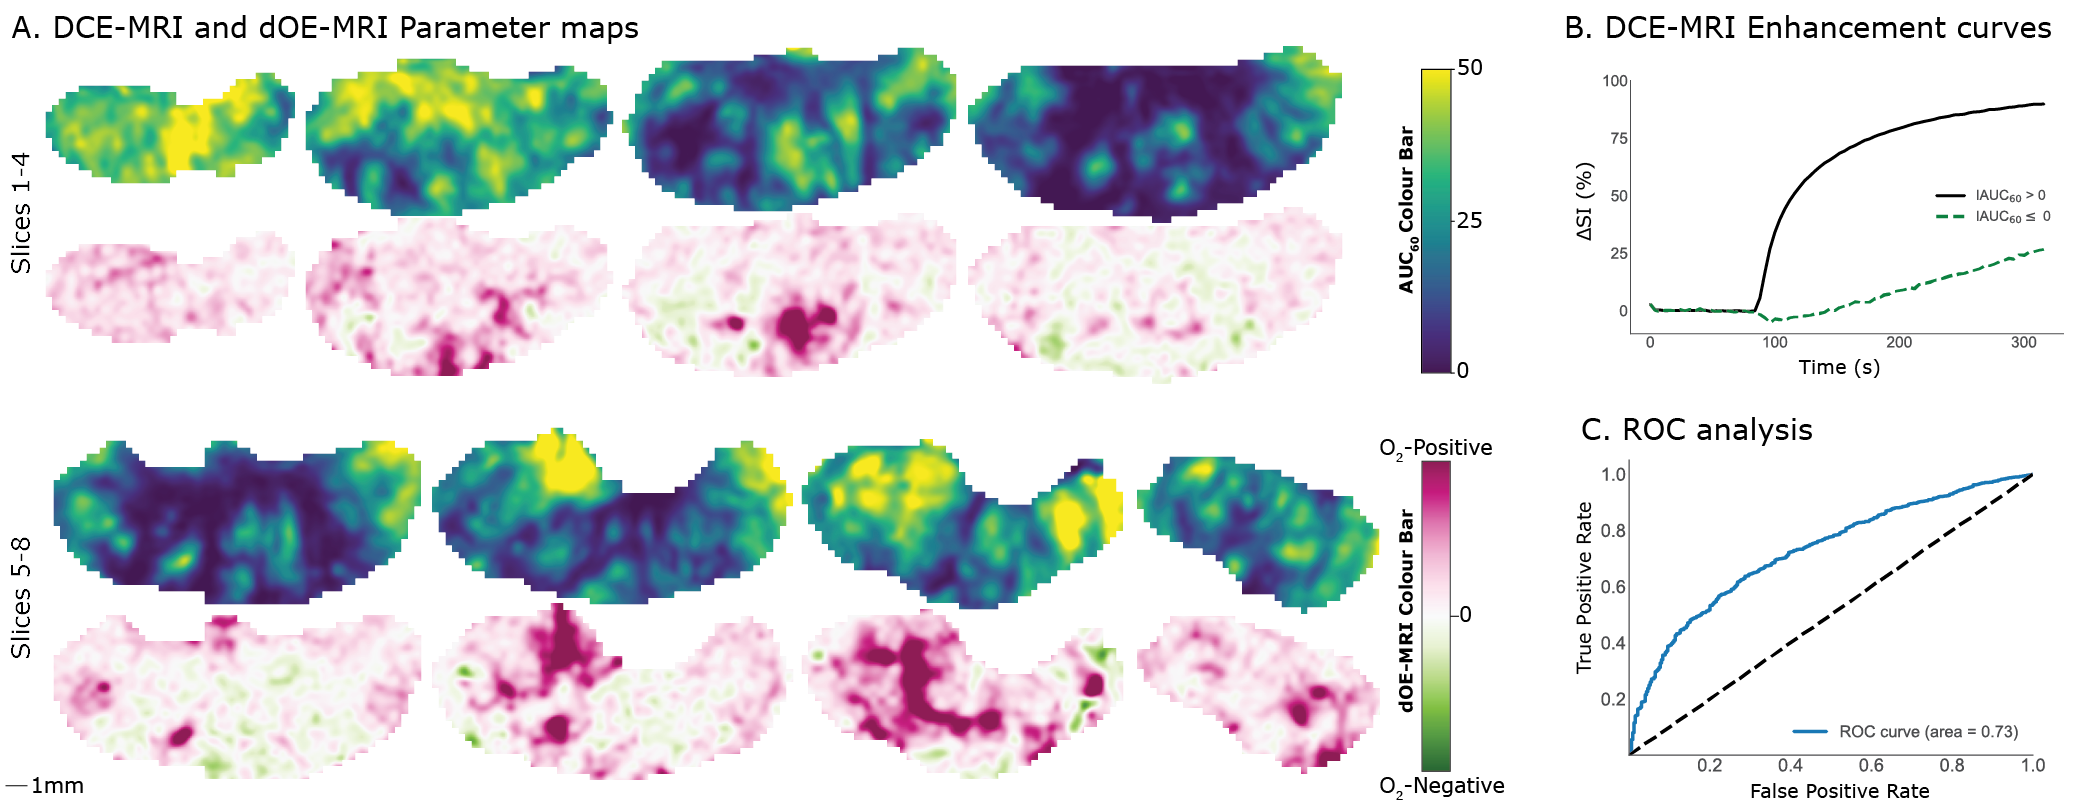
\includegraphics[width=\textwidth]{oemri/oemri-images/oemri_perfusion.png} % requires the graphicx package
   \caption{dOE-MRI maps and DCE-MRI AUC$_{60}$ maps of all slices of a tumour (A).
Signal enhancement curve of all perfused voxel and unperfused voxels (B).
A receiver-operator-characteristic (ROC) plot of a binary AUC$_{60}$ perfusion map and the dOE-MRI oxygen responsiveness map.
Area under the ROC curve was 0.73.}
   \label{perfusion}
\end{figure}

\subsection{dOEMRI maps correspond to matched histology sections}

Tumour tissue cryosections obtained to match MR imaging slices were stained to show vasculature and regions of pimonidazole-labeled hypoxia.
Pimonidazole staining is heterogeneously dispersed within regions of viable tissue containing tumour blood vessels for both SCCVII tumours, where vessels are depicted by perfusion marker carbocyanine in Figure~\ref{sccfigure}, and for HCT-116 tumours, where vessels are labeled with CD31 staining in Fig~\ref{hctfigure}.
In corresponding dOE-MRI maps for both tumour models O$_2$-positive voxels (purple) generally align with the most oxygenated regions of histology sections, where pimonidazole labeling is absent, however areas of mismatch are also observed.


\begin{figure}[htbp]
   \centering
   \includegraphics[width=\textwidth]{oemri/oemri-images/oemri_sccfigure.png} % requires the graphicx package
   \caption{SCCVII murine tumours with slice-matched histological, stained images shown next to the dOE-MRI parameter maps and the corresponding ICA extracted components.
Relatively oxygenated areas of tumour that are negative for pimonidazole (green)-labeled hypoxia in histology generally correspond to O2 positive (purple) areas of dOE-MRI maps.}
   \label{sccfigure}
\end{figure}

\begin{figure}[htbp]
   \centering
   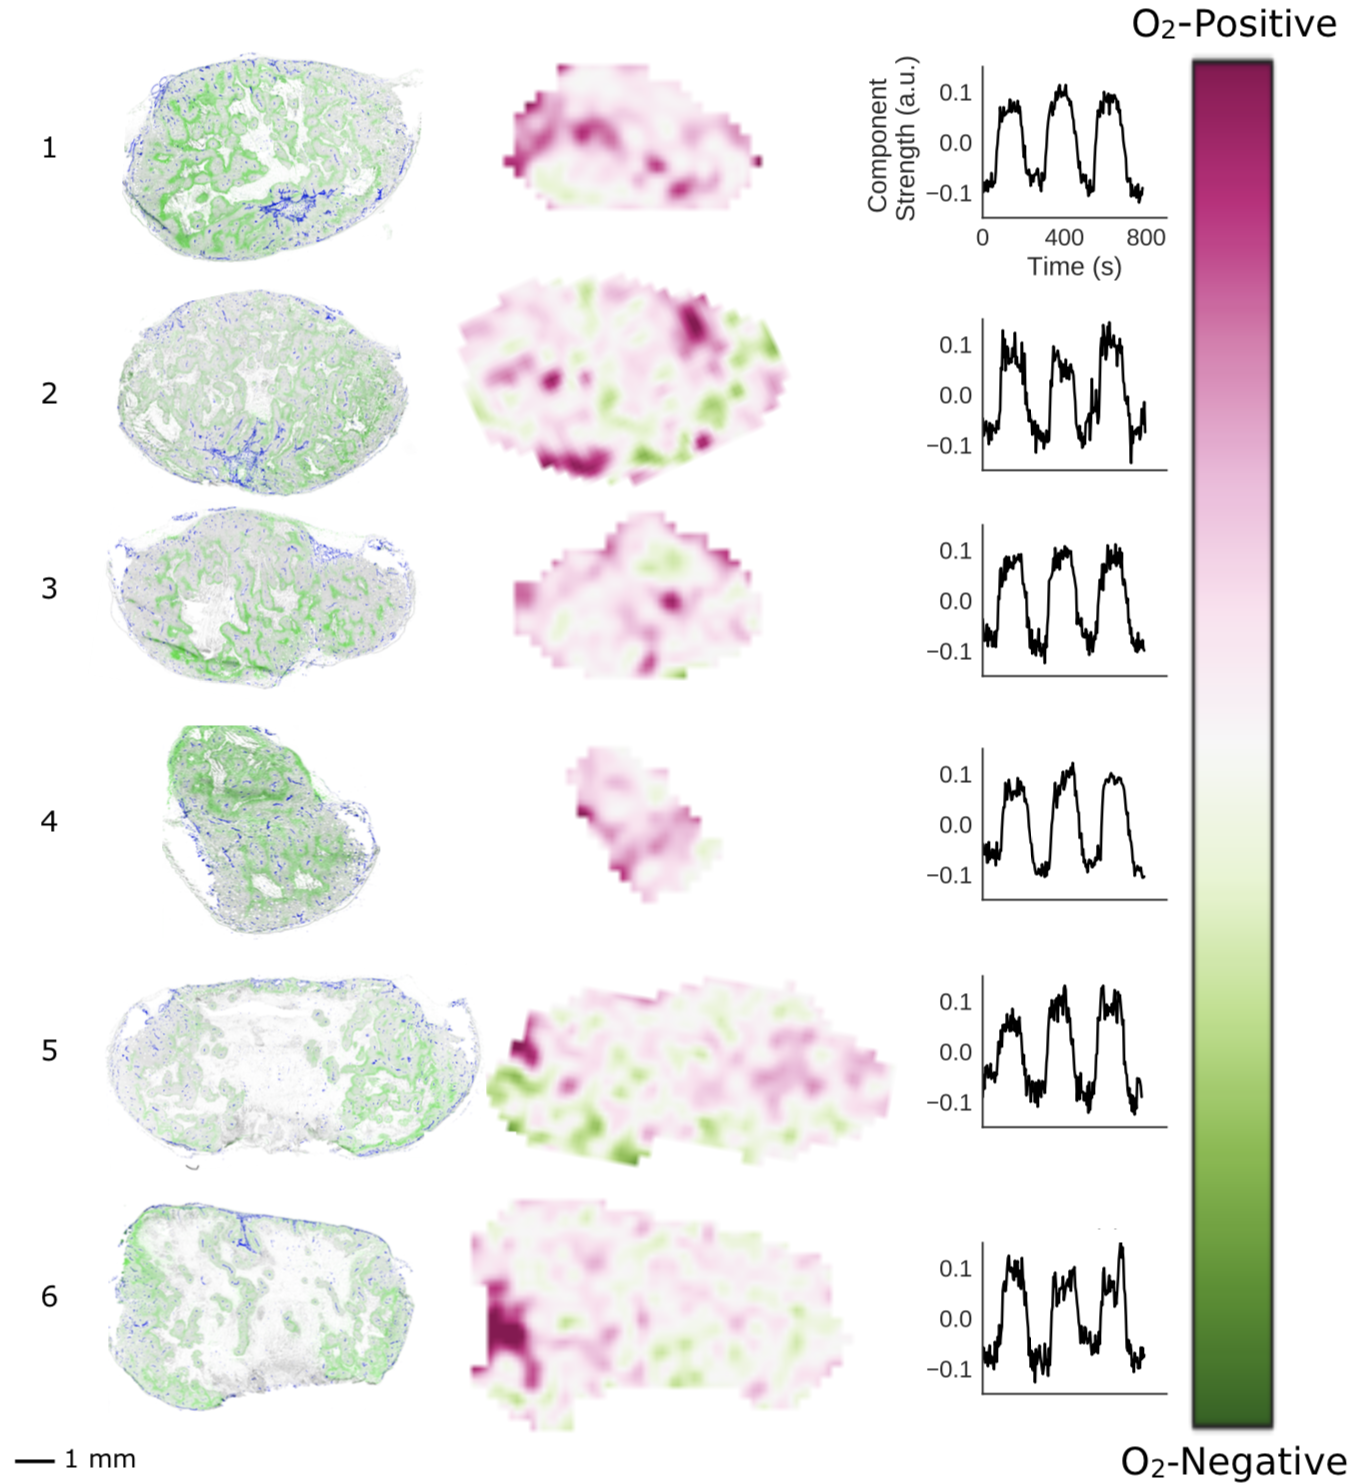
\includegraphics[width=\textwidth]{oemri/oemri-images/oemri_hctfigure.png} % requires the graphicx package
   \caption{HCT-116 human colorectal xenografts with slice-matched histological, stained images shown next to the dOE-MRI parameter maps and the corresponding ICA extracted components.}
   \label{hctfigure}
\end{figure}

% ======================================================================
\section{Discussion}
% ======================================================================

Early pioneering work by Young et al.
showed that oxygen acts as a paramagnetic contrast agent by demonstrating its ability to reduce T$_1$ upon inhalation~\cite{Young:1981vf}.
Subsequent efforts have included either acquisition of quantitative T$_1$ maps before and after oxygen breathing, or acquiring dynamic T$_1$w signal intensity images and calculating $\Delta$T$_1$ during periods of oxygen inhalation.
However, due to the small changes in T$_1$ that arise as oxygen dissolves in the plasma and interstitial fluids, T$_1$ maps have relatively poor sensitivity and, application of existing OE-MRI techniques is are limited to the most perfused tumour models.
For instance, O'Connor reported that in the highly perfused 786-0-R tumour lines, 85-96\% of all imaged tumour voxels were deemed to be oxygen-enhancing.
In those tumours, there was a good correlation between histological hypoxic fraction and oxygen refractory voxels.
However, in the more weakly perfused SW620 tumours where only 76\% of the voxels are oxygen-enhancing, there were no significant correlations with the histological hypoxic fraction.
To improve sensitivity and make OE-MRI more applicable in poorly perfused tumour models, companion DCE-MRI was then used to select only perfused voxels for oxygenation assessment.
Similarly, Linnik et al.
reported excellent correlation between percentage of ``negative AUC$_{OE}$'' ($O_2$-negative) voxels and percentage hypoxic areas in the highly vascular preclinical U87MG tumour xenografts~\cite{Linnik:2013hf}.
However, in the same study, glioblastomas in humans did not differentially enhance based on their OEMRI status; an effect attributed by the authors to the different perfusion characteristic of these clinical tumours.
Despite OE-MRI's limitations when applied to poorly perfused or oxygenated tumours, there is some evidence that clinically relevant tumour oxygenation can be measured.
Zhao et al. used a single-cycle carbogen challenge to evaluate oxygenation with T$_1$-w images and reported that the well-oxygenated Dunning prostate R3327-HI tumours showed a much larger response than the more hypoxic R3327-AT1 subline~\cite{Zhao:2015ez}.
Excitingly, they reported successful tumour stratification for radiation response based on oxygenation status in the same R3327-AT1 tumours~\cite{Hallac:2014cb}.
It seems evident that due to the small effect oxygen has on reducing T$_1$, a large proportion of the tumour must be oxygenated in order to assess oxygenation.

For dOE-MRI to receive wider clinical applicability, it would benefit from a greater sensitivity in a diverse range of tumour models, independent of their vascular density and perfusion status.
It would ideally also avoid the need for additional costly imaging with contrast agents.

Our method leverages two intrinsically linked techniques to achieve higher speed and greater sensitivity.
First, a cycling gas challenge is used to probe tissue response by introducing an independent signal modulation unrelated to nuisance contributions such as temperature drifts and motion.
A repeating gas challenge improves the detection sensitivity of small amplitude signal changes that are typical of oxygen-enhanced MRI.
	 Second, a repeating signal modulation enables further improved sensitivity through the use of ICA, a signal processing technique to isolate source signals - T$_1$-w changes due solely to the cycling oxygen - without knowledge of the response function (Figure~\ref{technique}).
While it is possible to generate correlation maps of the oxygen cycling paradigm with T$_1$-w signal changes that appear very similar to dOE-MRI maps, knowledge of the response function is required for this approach (Figure~\ref{correlation}).
As shown in Figure~\ref{correlation}, presupposing a particular oxygen response function biases the identification of responding O$_2$-positive voxels.

The improved sensitivity of our technique results in a broader applicability of dOEMRI: an oxygen-enhancing component was extracted successfully in all imaged xenografts across a range of tumour lines (Figure~\ref{versatile}) in over 60 mice.
We have established the reliability of the technique by comparing maps created from a temporally undersampled T1w time course to the map from the full three-oxygen-cycle time course.
This also suggested that the time course has sufficient SNR even at three-fold undersampling to successfully extract the oxygen responsive component (Figure~\ref{repeatability}).
Further, we have shown that individual cycles of the gas challenge can be assessed separately resulting in a minimum time of 6min to produce a dOE-MRI map.
This compares favourably with previous work requiring about 12min~\cite{Zhao:2015ez} to acquire $\Delta$SI oxygen-response maps and 15min~\cite{OConnor:2016ee} to create oxygenation binary maps.
Within the relatively short 14-minute imaging time examined, our data show only slight changes in the oxygenation maps between cycles.
Temporal oxygenation changes on the order of minutes can be assessed with dOEMRI by comparing correlation maps generated from sequential cycles to those from the undersampled time course.
This also provides a benchmark for future assessment of temporal characteristics of dOE-MRI maps.
In longer imaging sessions these same tumours may exhibit varying oxygenation patterns between cycles.
Periods of oxygen-starvation and re-oxygenation cycling in tumours has been termed cycling hypoxia and can arise for intermittent periods based on temporary vessel occlusions, or may be permanent acute changes in hypoxia~\cite{Dewhirst:2009de,Bayer:2011js}.
The clinical importance of intermittent hypoxia is unclear largely due to poor availability of techniques to measure it in the clinic~\cite{Michiels:2016hv}.
Recent work on measuring cycling hypoxia in patients using R$_2^*$~\cite{Panek:2017ge} shows that interest in this phenomenon continues.
dOE-MRI offers a versatile technique where the duration of the cycles and gas challenge, temporal resolution and desired signal-to-noise can be modified based on the imaging objectives, which could include investigating intermittent perfusion or intervention-mediated changes in the tumour microenvironment.

Of note, supplying excess oxygen to hypoxic tumour cells over time has the potential for increasing the baseline oxygen concentration, effectively reducing the hypoxic fraction and altering the tumour microenvironment~\cite{Linnik:2013hf}.
This would result in voxels becoming oxygen responsive over progressive oxygen cycles and would depend on the tumour characteristics as well as the duration of the oxygen challenge.
This was not observed on the timeline in our study when using ICA to extract changes in T$_1$-w signal intensity just due to the gas challenge, but should it arise in other contexts it could possibly be mitigated by extending the air-breathing part of the cycle.
The potential for creating a hyperoxia steady state by modulating oxygen duration is discussed in detail by Losert et al ~\cite{Losert:2002gt}.

Interestingly, our data suggests that dOE-MRI may have application as a surrogate imaging marker for assessing tumour perfusion without exogenous contrast agents.
O'Connor used an IAUC$_{60}$ map from DCE-MRI as a mask to obtain Oxy-R fractions that correlated well with histological hypoxic fraction~\cite{OConnor:2016ee}.
However, the binary oxygenation map was not compared to the perfusion map and merits further consideration.
In Figure~\ref{perfusion} while dOE-MRI maps are not perfectly matched by the DCE-MRI data, there is generally excellent agreement.
In all slices, all O$_2$-positive regions are definitely perfused, but not all perfused regions are O$_2$-positive.
Comparing AUC$_{60}$ unperfused regions to dOE-MRI maps is not as clear as these regions are either O$_2$-negative or non-responsive.
Should dOE-MRI indeed be found as an applicable biomarker in some scenarios, this would present an exciting improvement over the more invasive DCE-MRI.

Typically, histological validation of MR data is done by collapsing rich histology data into a single metric, such as a hypoxic fraction, with whole-tumour or single-slice average comparisons.
While this is a useful validation approach, it is worthwhile to note that hypoxia in particular is a difficult target to validate.
Tumour oxygenation exists as a spectrum ranging from normoxic, at levels similar to neighbouring normal tissues of origin, to hypoxic.
What is of interest in the oncology community is \emph{clinically relevant} hypoxia~\cite{Horsman:2012kw}.
This refers to measurable tumour oxygenation levels that are biomarkers of physiologically meaningful phenomena, including patient prognosis or tumour sensitivity to treatment.
Pimonidazole has been demonstrated as a clinically relevant marker of hypoxia, but poor correlation with pimonidazole does not exclude other measures of tumour oxygenation from potential utility.

Measurable pimonidazole-adduct formation occurs when the O$_2$ tension in the vicinity drops below 10 mmHg but in dOE-MRI, O$_2$-positive voxels are extracted as excess oxygen dissolves in the plasma and interstitial tissue fluid to decrease T$_1$.
Voxels where T$_1$ has statistically significantly increased have previously been correlated to poorly perfused regions~\cite{Linnik:2013hf} but the exact mechanism for a T$_1$ increase as a result of oxygen inhalation has not yet been confirmed~\cite{Zhao:2015ez, OConnor:2016ee}.
O$_2$-positive regions in dOE-MRI maps are generally in good agreement with well perfused areas of histology images for both HCT-116 and SCCVII tumours, as shown in Figures~\ref{sccfigure} and~\ref{hctfigure}.
Voxels exhibiting signal reduction with the O$_2$ stimulus (=O$_2$-negative, green) typically correspond with pimonidazole staining but not all pimonidazole-labeled regions are shown as O$_2$-negative.
Mismatches may be attributed to the different sensitivities and detection thresholds of hypoxia/oxygenation of pimonidazole and dOE-MRI.
Future work to evaluate the utility of dOE-MRI will ultimately depend on its context-dependent validation as a relevant measure of tumour hypoxia.
In a promising study, White et al.
has shown that OE-MRI may be very relevant in developing prognostic factors to predict tumour response to hypofractionation by stratifying tumours that may benefit from oxygen breathing during irradiation~\cite{White:2016fz}.

An important limitation of this study is the absence of a quantitative metric to assess the absolute oxygenation of tumours in O$_2$-negative areas.
This is largely due the competing effects of T$_1$ and T2* shortening on the signal intensity, an issue similar to that reported by others~\cite{Remmele:2012df,Burrell:2013je,Linnik:2013hf}.
O$_2$-positive and O$_2$-negative fractions can be obtained from dOE-MRI ICA component maps by deploying groupICA techniques {refs} or setting significance thresholds using a t-test and computing z-scores.

To help understand the oxygen dynamics in tumours, including the effect of hemoglobin with T$_2^*$ mapping, fitting exponential recovery and decay curves to the extracted oxygen response curves may provide additional insights as originally proposed by Losert et al.
in the brain~\cite{Losert:2002gt}.
We hope to expand dOE-MRI by developing a quantitative metric that can be used to dynamically characterize the clinically relevant oxygen status of tumours, relating this information to treatment sensitivities and outcomes.

% ======================================================================
\section{Conclusions}
% ======================================================================

In this study we extended existing oxygen-enhanced MRI techniques by adding a cycling element to the respiratory challenge and using a blind-source separation signal processing technique (ICA) to extract oxygen responding voxels.
This method presents significant improvements to the sensitivity and applicability of dOE-MRI, making it more clinically accessible.
ICA-assisted dOE-MRI is easy to implement as the sequence acquisition is relatively short, does not require a contrast agent and most centres already have access to dynamic T$_1$ weighted MRI acquisitions that many patients already routinely receive.
Using our dOE-MRI technique, the small changes in T$_1$ weighted signal intensity arising from the respiratory challenge can be separated robustly, while common quantitative T$_1$ mapping methods such as determining $\Delta$ T$_1$ using the Look-Locker technique have poor consistency and sensitivity.
We have also shown the potential utility of dOE-MRI for measuring temporal changes in oxygenation and as a contrast agent-independent surrogate for vascular perfusion.
dOE-MRI is an exciting, non-invasive and widely available technique for assessing tumour oxygenation that could provide a crucial tool in the field of radiation oncology and in the development of treatments targeting the tumour microenvironment.
  

% ======================================================================
\section{Acknowledgments}
% ======================================================================

This work was supported by NSERC and CIHR.
Thanks to Dr.
Martin McKeown (sp) for this help


\endinput

Any text after an \endinput is ignored.
You could put scraps here or things in progress.
